  {\large \fontB Description:}
  
  {\bf solHy} is a 3-dimensional analytical solution to the Cauchy equations with the acceleration term set to zero
  to represent creeping flow. The boundary conditions are free-slip everywhere on a unit domain. 
  The flow is driven by a dense column in one corner. The output from the code is a two-dimensional slice
  in the $z - x$ plane at a given coordinate $y$.
  \\

  {\large \fontB Parameters:}
 
  The variable parameters of this solution are:
  \begin{itemize}
    \item{density parameter: $ \sigma $.}
    \item{viscosity: $\eta$.}
    \item{x width of dense block: $dx$.}
    \item{y width of dense block: $dy$.}
    \item{y coordinate of 2D slice: $y$.}
    \end{itemize}

  \begin{SCfigure}[][h]
    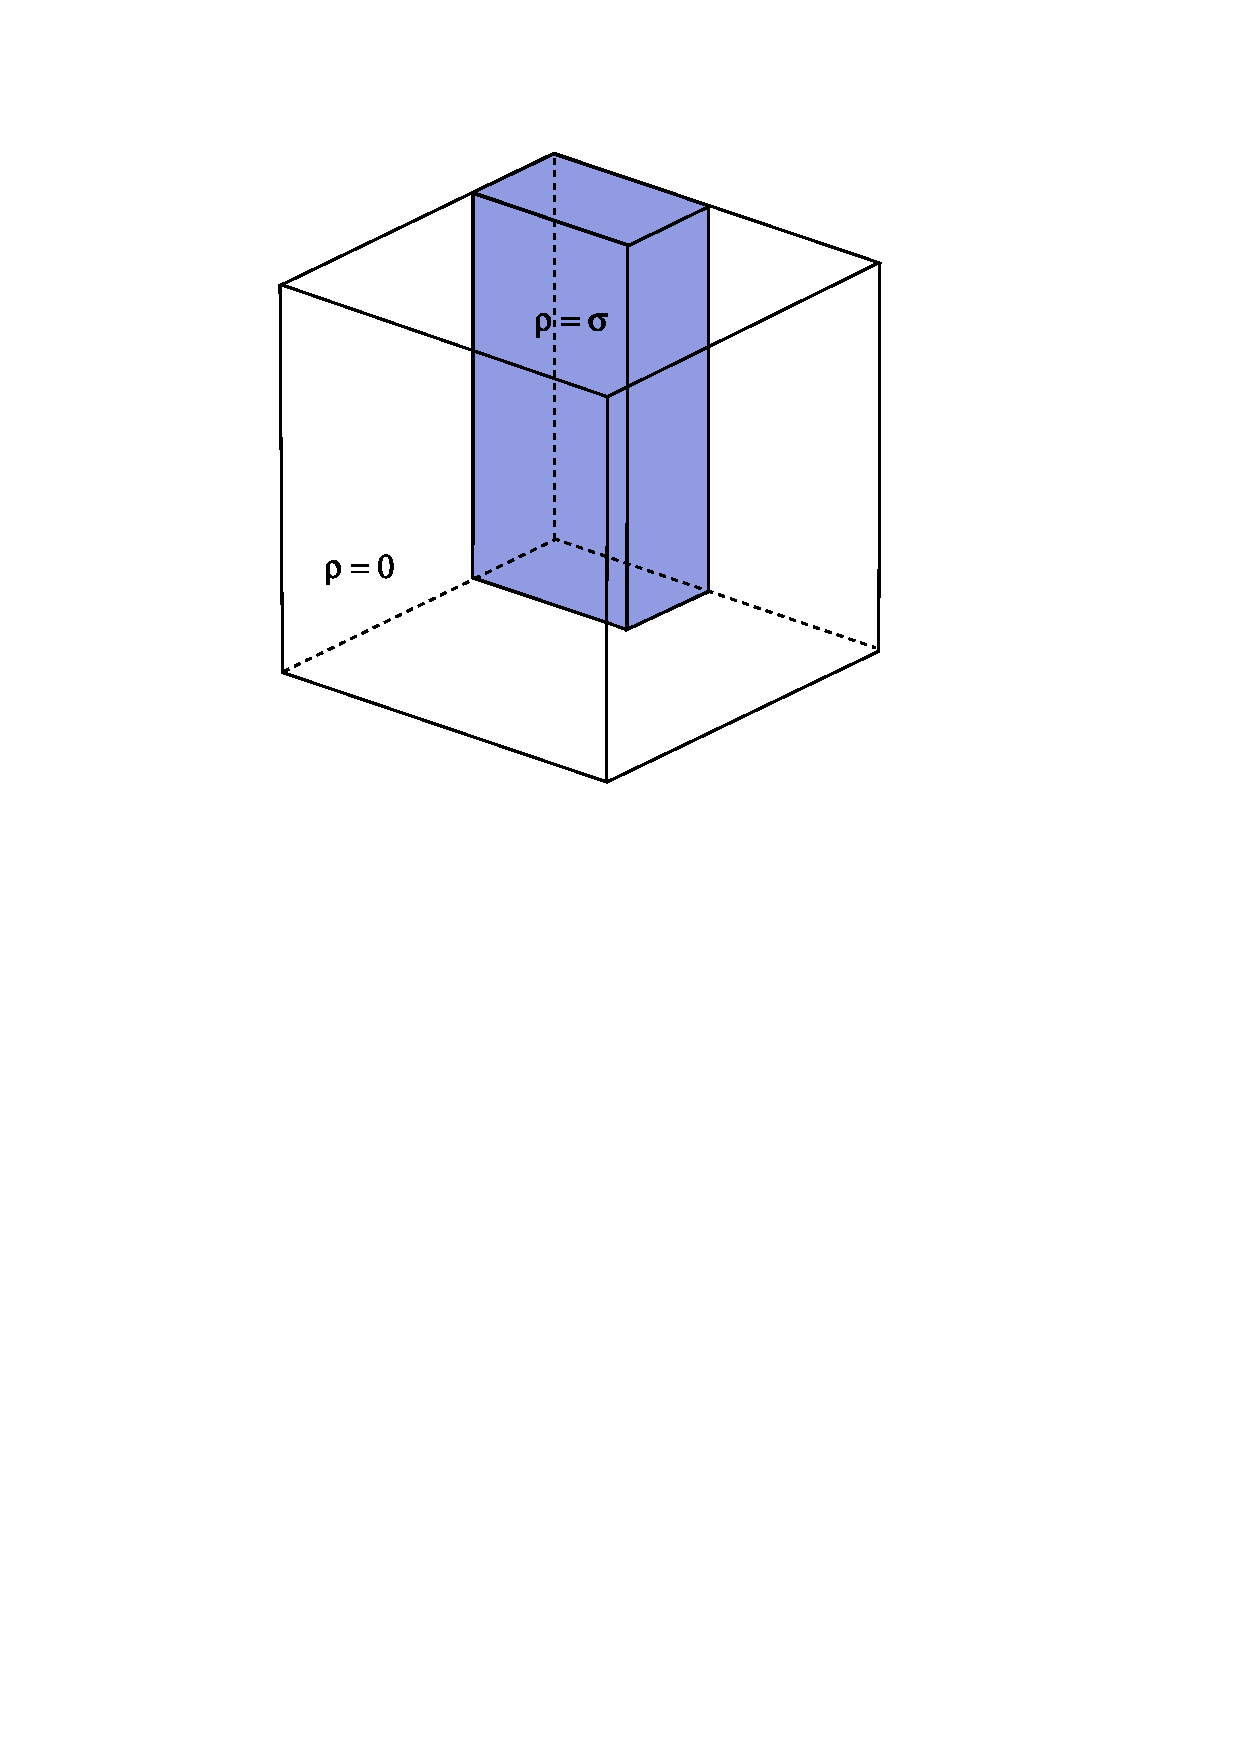
\includegraphics[width=6cm,clip]{../figs/figH}
    \caption[Short caption]{\label{figHy} 
      Solution ({\bf SolHy}):
      This solution has a block of density $\rho = \sigma$
       from $ 0 < x < dx $ and $ 0 < y < dy $ extending in the $z$ direction.
      The boundary conditions are free slip everywhere on the surfaces of the unit box.}
  \end{SCfigure} 
  

